%%
%% Author: Dario Chinelli
%% begin 2019-12-04
%% last mod 2022-02-02
%%

% Preamble
\documentclass[class=article, crop=false]{standalone}

% Packages
\usepackage[subpreambles=true]{standalone}
\usepackage{import}
\usepackage{graphicx}
\usepackage{amsmath}

% Document
\begin{document}

% \subsection{Metaforum}

% \subsection{Train field 7}

% \subsection{Glow experiment}

\paragraph{Utrecht Centraal (Floorefield 10)}
The datas analyzed in this work are given as a CSV file and come from a collaboration with the \emph{ProRail company}.
Specifically this data were collected at the Utrecht’s train station during one day.
The (Figure \ref{fig:trainf10}) shows the camera’s point of view of the analyzed field.
This spot offers a great multitude of path's type, due to its \emph{morphology}. 
It is a rectangular base field, where there are a few obstacle and a lot of entrance and exits.
This field is both a corridor from two zones of the station and a cross zone. 
It also as more than one shops where people may entry to or exit from it.
This complex scenario permit to strongly compare all the four models to each others and with the real datas.

\begin{figure}[h]
\centering
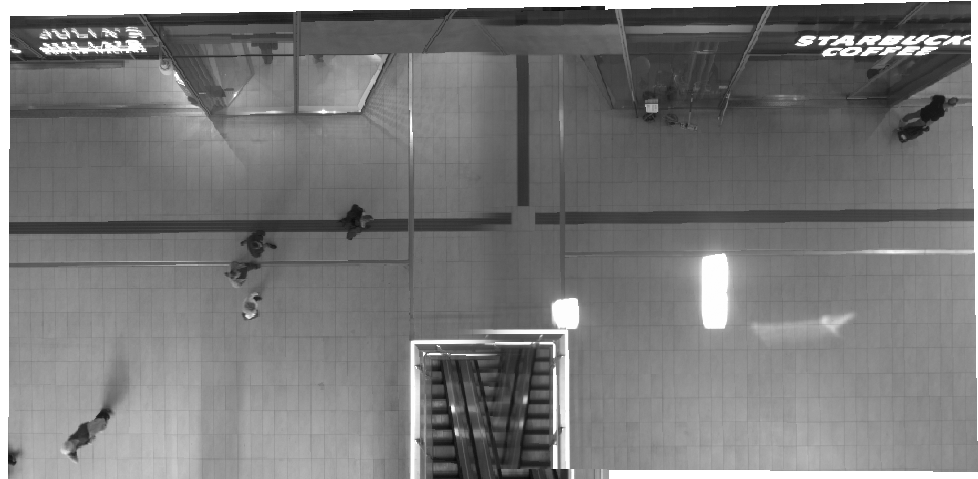
\includegraphics[width=0.4\textheight]{imgs/bg10.png}
\caption{Utrecht Centraal, cameras point of view (Floorfield 10)}
%\cite{bibliography}
\label{fig:trainf10}
\end{figure}



\end{document}